%Tabela de resultados de adições em um corpo GF($2^4$)

\thispagestyle{fancy}
\renewcommand{\thesubsection}{\Alph{section}}
\section{Padrões de subamostragem da  crominância}
\label{cro_diz}

Para especificar a forma de subamostragem da crominância utiliza-se a representação j:a:b, em que cada letra significa:
\begin{itemize}
\item $j$: número de pixels de referência da luminância que possuem informações provenientes do processo de aquisição.
\item $a$: número de pixels dos canais Cb e Cr de $j$ na horizontal que possuem informações provenientes do processo de aquisição.
\item $b$: número de pixels dos canais Cb e Cr de $a$ na vertical que possuem informações provenientes do processo de aquisição.
\end{itemize}

\section{Formatos mais comuns}

Há diferentes formas de subamostragem da crominância, cada uma voltada para alguma de aplicação espefícica. As mais comuns são listadas a seguir.

\subsection{4:4:4}

Este padrão consiste na preservação das três componentes Y'CbCr obtidas pelo processo de aquisição de imagem, portanto não há subamostragem da crominância.

\subsection{4:2:2}

Neste formato a amostragem horizontal da crominância é reduzida pela metade enquanto que a amostragem na vertical é mantida.

\subsection{4:2:0}

Neste formato a amostragem em ambas as direções da crominância é reduzida pela metade.


\begin{figure}[!ht]
\begin{center}
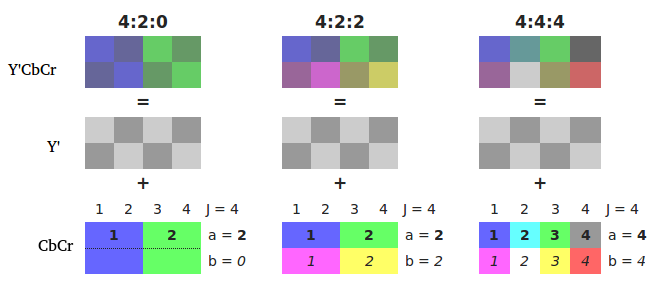
\includegraphics[scale=0.5]{./Figures/png/subamostragem.png}
\caption{Formatos mais comuns de subamostragem da crominância.}
\label{fig:subamostragem}
\end{center}
\end{figure}
